% Make nice A4 pages for print:
%\usepackage{pgfpages}
%\pgfpagesuselayout{resize to}[a4paper,border shrink=5mm,landscape]

\beamertemplatenavigationsymbolsempty

\setbeamertemplate{bibliography item}[text]

\usepackage[type={CC},modifier={by-sa},version={4.0}]{doclicense}

\usepackage[utf8]{inputenc}
\usepackage{hyperref}
\usepackage{breakurl}
\usepackage{graphicx}
\usepackage{pgfplots}
\usepackage{pgf}
\usepackage{tikz}
\usetikzlibrary{positioning}
\usetikzlibrary{arrows}
\usetikzlibrary{decorations.markings}
\usetikzlibrary{calc}
\usetikzlibrary{matrix}
\usetikzlibrary{shapes}
\usetikzlibrary{decorations.pathmorphing}
\usetikzlibrary{fit}
\usetikzlibrary{backgrounds}
\usetikzlibrary{plotmarks}
\usepackage{stmaryrd}
\usepackage{listings}
\usepackage{pdflscape}
\usepackage{perpage}
\usepackage{appendixnumberbeamer}

%\usepackage[thmmarks,amsmath,amsthm]{ntheorem} % already included in beamer
\usepackage{thm-restate}

\usepackage[sort&compress,numbers]{natbib}  % to be have \citet, \citeauthor, \citeyear

\MakePerPage{footnote}

\tikzstyle{o}=[r,ppBlue]
\tikzstyle{r}=[thick,rectangle,align=center]
\tikzstyle{t}=[r,ppTrans] %,font=\bfseries]
\tikzstyle{dd}=[densely dashed]
\tikzstyle{n}=[r,ppBlue]
\tikzstyle{p}=[r,ppRed]
\tikzstyle{ppRed}  =[draw=red,  fill=  red!20]
\tikzstyle{ppBlue} =[draw=blue, fill= blue!20]
\tikzstyle{ppGreen}=[draw=green,fill=green!20]
\tikzstyle{ppTrans}=[draw=none, fill=none]

\usetheme{Warsaw}

\useoutertheme[subsection=true]{smoothbars}
%\useoutertheme[subsection=false]{miniframes}

\definecolor{bblue}{HTML}{D7DF01}	% yellow-ish actually, for better black/white printing
\definecolor{rred}{HTML}{C0504D}
\definecolor{ggreen}{HTML}{9BBB59}
\definecolor{ppurple}{HTML}{9F4C7C}
\definecolor{lightgray}{rgb}{0.3,0.3,0.3}
\definecolor{lightergray}{rgb}{0.9,0.9,0.9}
\definecolor{UniBlue}{RGB}{83,121,170}

\DeclareTextFontCommand\textintro{\normalfont\bfseries\itshape} % nice!
\newcommand{\intro}[2][]
{%
	\textintro{#2}%
}
\newcommand{\empha}[2][]
{%
	\emph{#2}%
}

%\theoremstyle{plain}
\newcounter{reqcounter}
\newtheorem{requirement}[reqcounter]{Requirement}

%setbeamercolor{structure}{fg=violet}

\makeatletter
\def\th@task{%
    \normalfont % body font
    \setbeamercolor{block title example}{bg=orange,fg=white}
    \setbeamercolor{block body example}{bg=orange!20,fg=black}
    \def\inserttheoremblockenv{exampleblock}
  }
\makeatother

\theoremstyle{task}
\newtheorem{task}{Task}

\newenvironment{assignment}%
{%\setbeamercolor{background canvas}{bg=violet}%
%\setbeamercolor{structure}{fg=cyan!90!black}%
 \setbeamercolor{frametitle}{bg=orange,fg=white}
\begin{frame}}%
{\end{frame}}%

\AtBeginSection[]{
  \begin{frame}
  \vfill
  \centering
  \begin{beamercolorbox}[sep=8pt,center,shadow=true,rounded=true]{title}
    \usebeamerfont{title}\insertsectionhead\par%
  \end{beamercolorbox}
  \tableofcontents
  \vfill
  \end{frame}
}




\pgfplotsset{compat=1.14}
\author{Markus Raab}


\date{13.03.2019}

\begin{document}

\renewcommand{\enquote}[1]{\emph{``#1''}} % Cannot be done earlier

%%%%%%%%%%%%%%%%%%%%%%%%%%%%%%%
\begin{frame}
	\titlepage
	\doclicenseThis
\end{frame}

%%%%%%%%%%%%%%%%%%%%%%%%%%%%%%%%%%%%%%%%%% 
\section{Problem}
{
\shadowcolor{black}
\shadowoffset{0.5pt}
\usebackgroundtemplate{\includegraphics[width=\paperwidth]{pics/clouds.jpg}}%
\begin{frame}
	\frametitle{\shadowtext{Misconfiguration}}
	\begin{itemize} %[<+->]
		\item   \textcolor{white}{\shadowtext{\empha[misconfiguration]{misconfigurations}~\cite{yin2011empirical,su2007autobash,attariyan2010automating,xu2015systems} are a major cause}}\\
			\textcolor{white}{\shadowtext{of system failures~\cite{wool2004quantitative,oppenheimer2003internet,pertet2005causes}}}
		\item   \textcolor{white}{\shadowtext{much time needed to fix misconfigurations~\cite{rabkin2011static,oppenheimer2003internet,yin2011empirical,mahajan2002bgp}}}
%		\item   \textcolor{white}{\shadowtext{configuration is a user interface for both developers}}\\
%			\textcolor{white}{\shadowtext{and system administrators}}
		\item   \textcolor{white}{\shadowtext{currently configuration is error-prone and under-specified}}
	\end{itemize}
\end{frame}
}

\section{Elektra}

\begin{frame}
	\frametitle{Elektra}
	\begin{itemize} %[<+->]
%		\item \citet{holland2001nofutz}~defined \empha{futzing} to denote \enquote{tinkering or fiddling experimentally}
%		\item With \intro[no-futz computing]{no-futz computing} \citet{holland2001nofutz} mean \enquote{that futzing should be allowed, but should never be required}
		\item \elektra{} is a framework implementing a modular \intro{configuration specification language} for configuration settings
		%\item In \elektra{} we use properties to specify configuration settings and configuration access
		\item \elektra{} enables \intro[no-futz computing]{no-futz computing} \cite{holland2001nofutz},
			i.e., error-prone \enquote{tinkering or fiddling experimentally} \enquote{should be allowed, but should never be required}
	\end{itemize}
\end{frame}

\begin{frame}
	\frametitle{Requirements of Elektra}

	\begin{itemize}
	\item formal
	\item extensible and flexible
	\item external to applications
	\item open for introspection (for tooling)
	\item enables (code) generation
	\end{itemize}
\end{frame}

\subsection{Metalevels}

\begin{frame}
	\frametitle{Metalevels}
	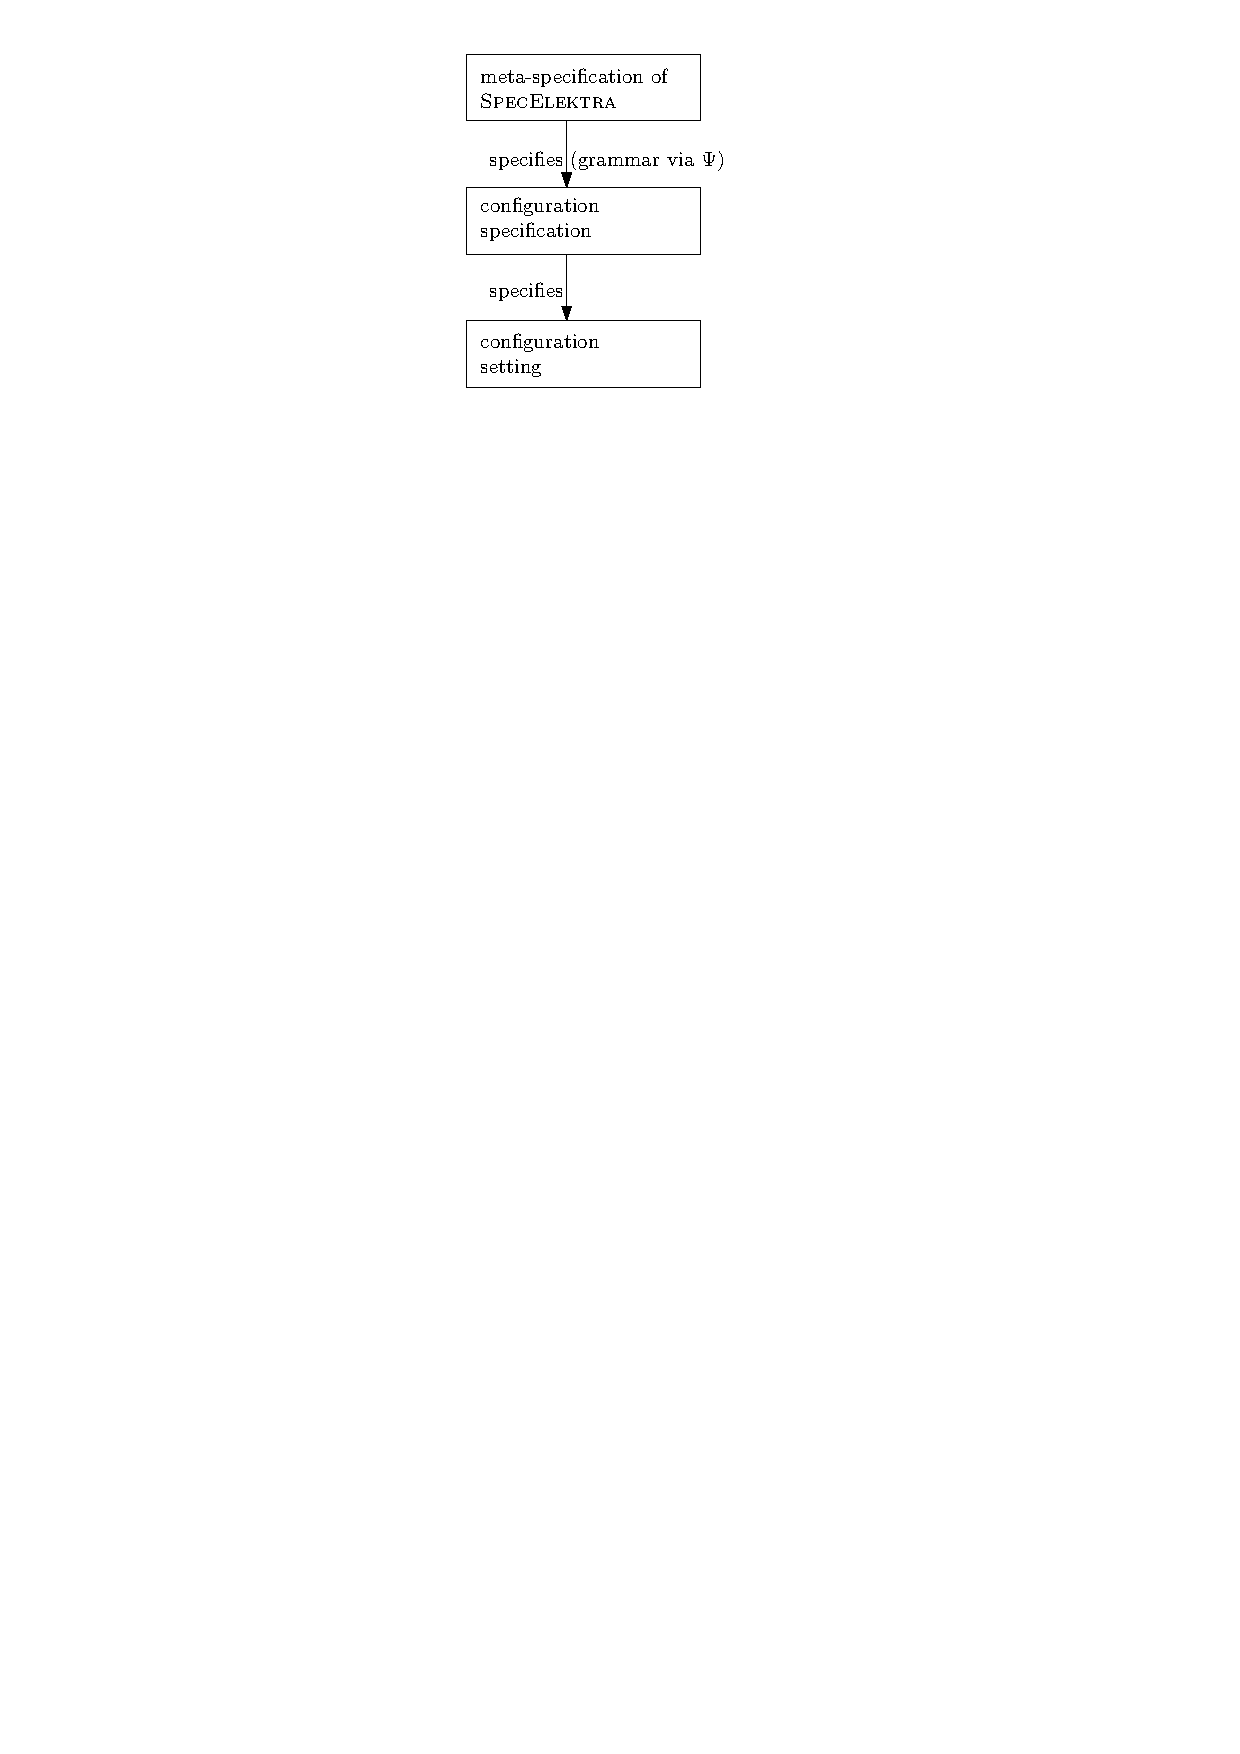
\includegraphics{metalevels}

	We will now walk through metalevels bottom-up.
\end{frame}

\begin{frame}[fragile]
	\frametitle{Configuration Settings}

	A configuration file may look like:

	\begin{code}[language=CfgElektra]
	a=5
	b=10
	c=15
	\end{code}

	We apply these configuration settings imperatively using:

	\begin{code}[language=bash]
	kdb set /a 5
	kdb set /b 10
	kdb set /c 15
	\end{code}

	And we list them with \lstinline[language=bash,morekeywords={ls},showspaces=no]^kdb ls /^.
\end{frame}

\begin{frame}[fragile]
	\frametitle{Specifications}
	For specifications such as:

	\begin{code}
	[slapd/threads/listener]
	  check/range:=1,2,4,8,16
	  default:=1
	\end{code}

	We apply the specifications imperatively using:

	\begin{code}[language=bash,morekeywords={meta-set}]
	kdb meta-set /slapd/threads/listener\
		check/range 1,2,4,8,16
	kdb meta-set /slapd/threads/listener\
	       	default 1
	\end{code}
\end{frame}

\begin{frame}[fragile]
	\frametitle{Meta-Specifications}
	For meta-specifications such as:

	\small
	\begin{code}
	[visibility]
	type:=enum critical important user\
	      advanced developer debug disabled
	description:=Who should see this\
	     configuration setting?
	\end{code}

	We apply the meta-specifications imperatively using:

	\begin{code}[language=bash,morekeywords={meta-set}]
	kdb meta-set /elektra/meta/\
		visibility type enum ...
	kdb meta-set /elektra/meta/\
		visibility description "Who ...
	\end{code}
\end{frame}


\begin{frame}[fragile]
	\frametitle{KeySet Generation}
	\begin{alertblock}{Idea}
	Use configuration file format grammar to describe both configurations and (meta-)specifications
	\end{alertblock}
	\pause

	\begin{grammar}
	<KeySet> ::= \lq ksNew'\WhiteSpace(' \{ <Key> \lq , \LineBreak'  \}  \{ \lq\WhiteSpace' \} \lq KS\_END);'

	<Key> ::= \lq keyNew \WhiteSpace ('' ' <key name> \lq ''  , \LineBreak' [ <Value> ] <properties> \lq KEY_END)'

	<Value> ::=  \{ \lq\WhiteSpace' \} \lq KEY\_VALUE, \WhiteSpace '' ' <configuration value> \lq ''  , \LineBreak'

	<properties> ::= \{ \{ \lq\WhiteSpace' \} <property> \lq , \LineBreak' \}

	<property> ::=  \lq KEY\_META, \WhiteSpace " ' <property name> \lq "  , \WhiteSpace " ' <property value> \lq " '
	\end{grammar}
\end{frame}

\begin{frame}[fragile]
	\frametitle{Example}
	\begin{example}
	Given the key ^spec:/slapd/threads/listener^, with the configuration value ^4^ and the property $\property{default} \mapsto 1$, \elektra{} emits:

	\begin{code}[gobble=4,language=Cpp]
	ksNew (keyNew ("spec:/slapd/threads/listener",
		       KEY_VALUE, "4",
		       KEY_META, "default", "1",
		       KEY_END),
	       KS_END);
	\end{code}
	\vspace{-1em}
	\end{example}

	\pause
	\begin{alertblock}{Finding}
	We have source code representing the settings.
	And if we instantiate it, we have a data structure representing the settings.
	Plugins emitting such ``configuration files'' are code generators.
	\end{alertblock}
\end{frame}

\begin{frame}
	\frametitle{Possible Properties}
	For example, SpecElektra has following properties:
	\begin{description}
	\item[type] represents the type to be used in the emitted source code.
	\item[opt] is used for short command-line options to be copied to the namespace \namespace{proc}.
	\item[opt/long] is used for long command-line options, which differ from short command-line options by supporting strings and not only characters.
	\item[restrict/write] yields compilation errors when developers assign a value to a contextual value within the program.
	\item[default] enables us to start the application even if the backend does not work.
	\end{description}
\end{frame}

\begin{frame}[fragile]
	With the specification:
	\par
	\begin{code}[gobble=4]
	[foo/bar]
	  default:=Hello
	  type:=string
	  opt:=b
	  restrict/write:=1
	\end{code}
	\par
	\elektra{Gen} gives the user read-only access to the object ^env.foo.bar^:
	\par
	\begin{code}[language=Cpp]
	std::cout << env.foo.bar;
	env.foo.bar = "Other world"; // comp. error
	\end{code}
	\par
\end{frame}

% hack: needed to render graphics properly
\begin{frame}<0>[noframenumbering]
	\begin{columns}[c]
	\begin{column}{7cm}
	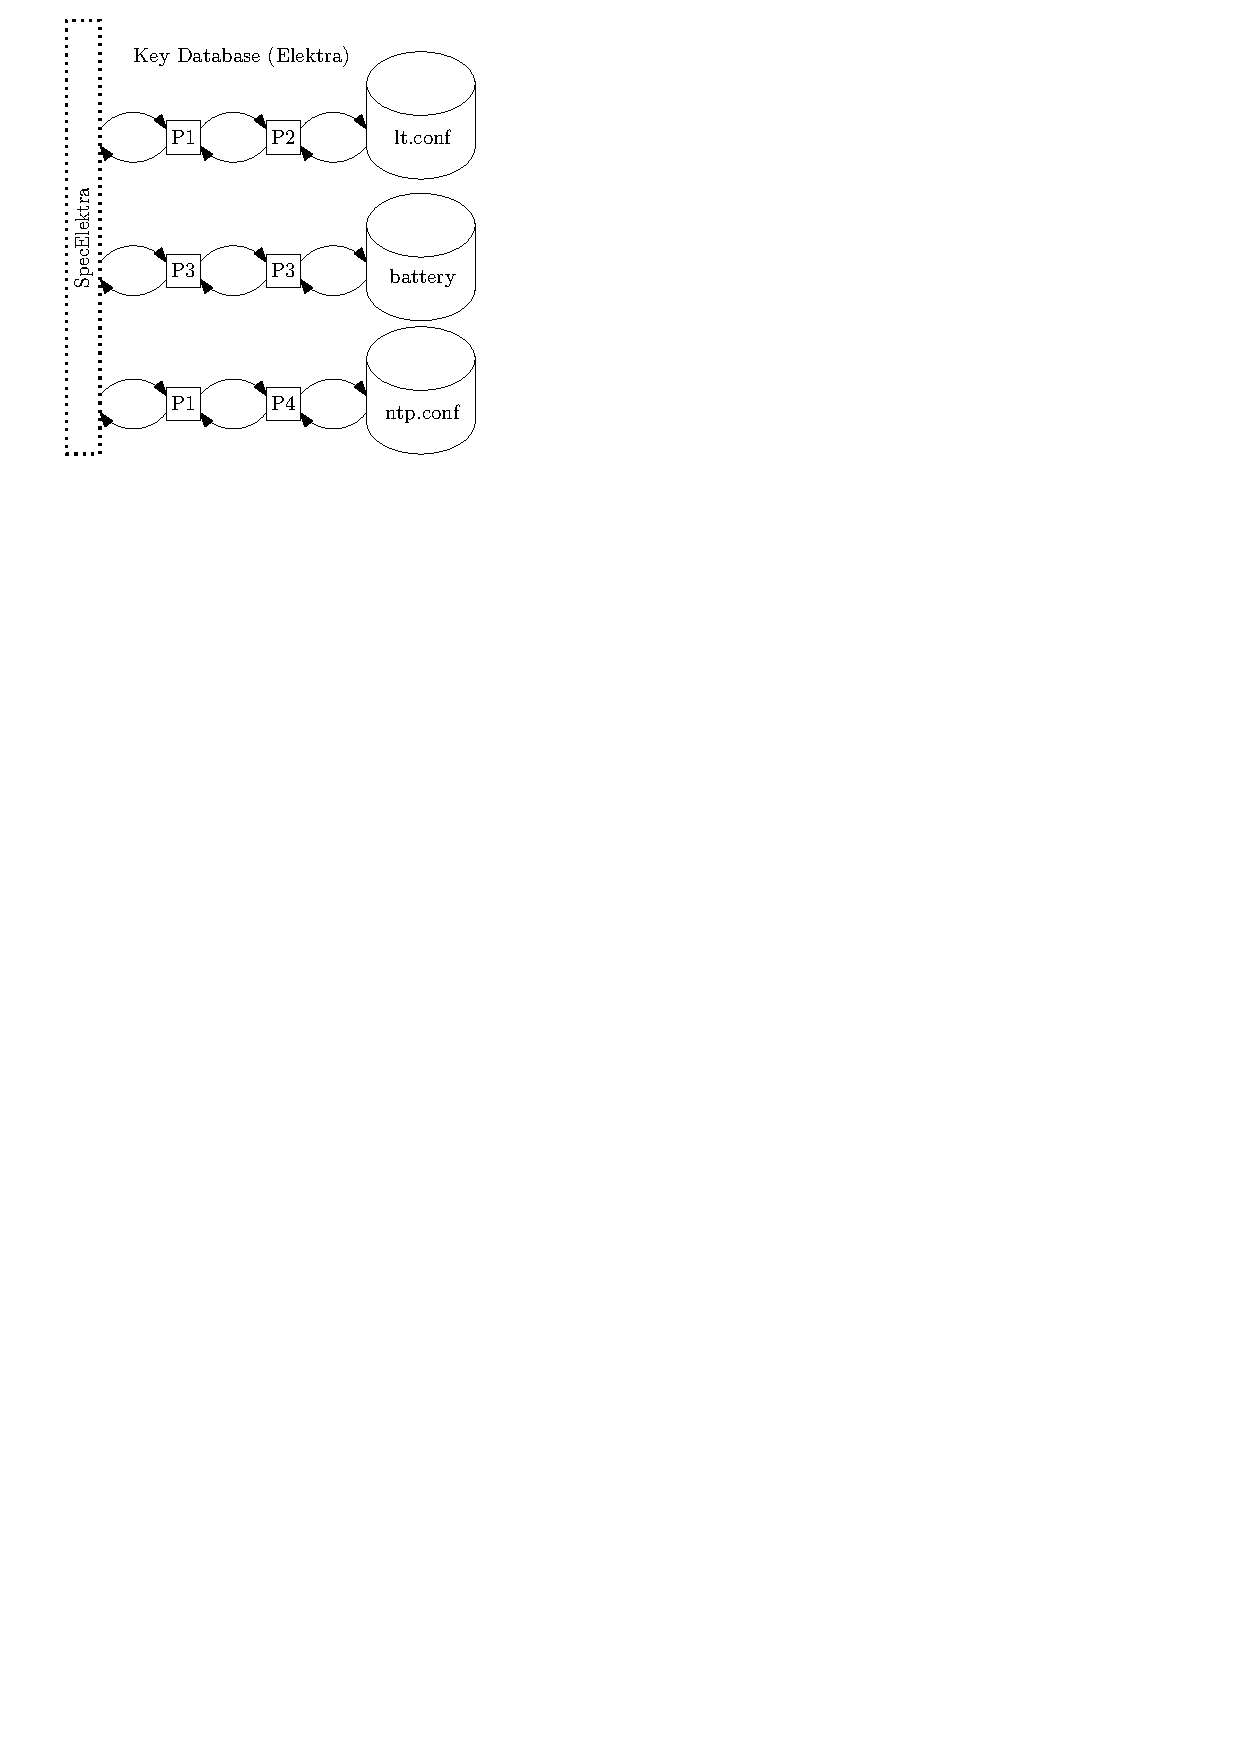
\includegraphics[scale=0.8]{horizontalmodularity}
	\end{column}
	\begin{column}{4cm}
	Cylinders are configuration files, P? are plugins~\cite{raab2016improving}.

	Key ideas:
	\begin{itemize}
	\item all work is done by plugins
	\item central data structure implements semantics
	\end{itemize}
	\end{column}
	\end{columns}
\end{frame}

\begin{frame}
	\begin{columns}[c]
	\begin{column}{7cm}
	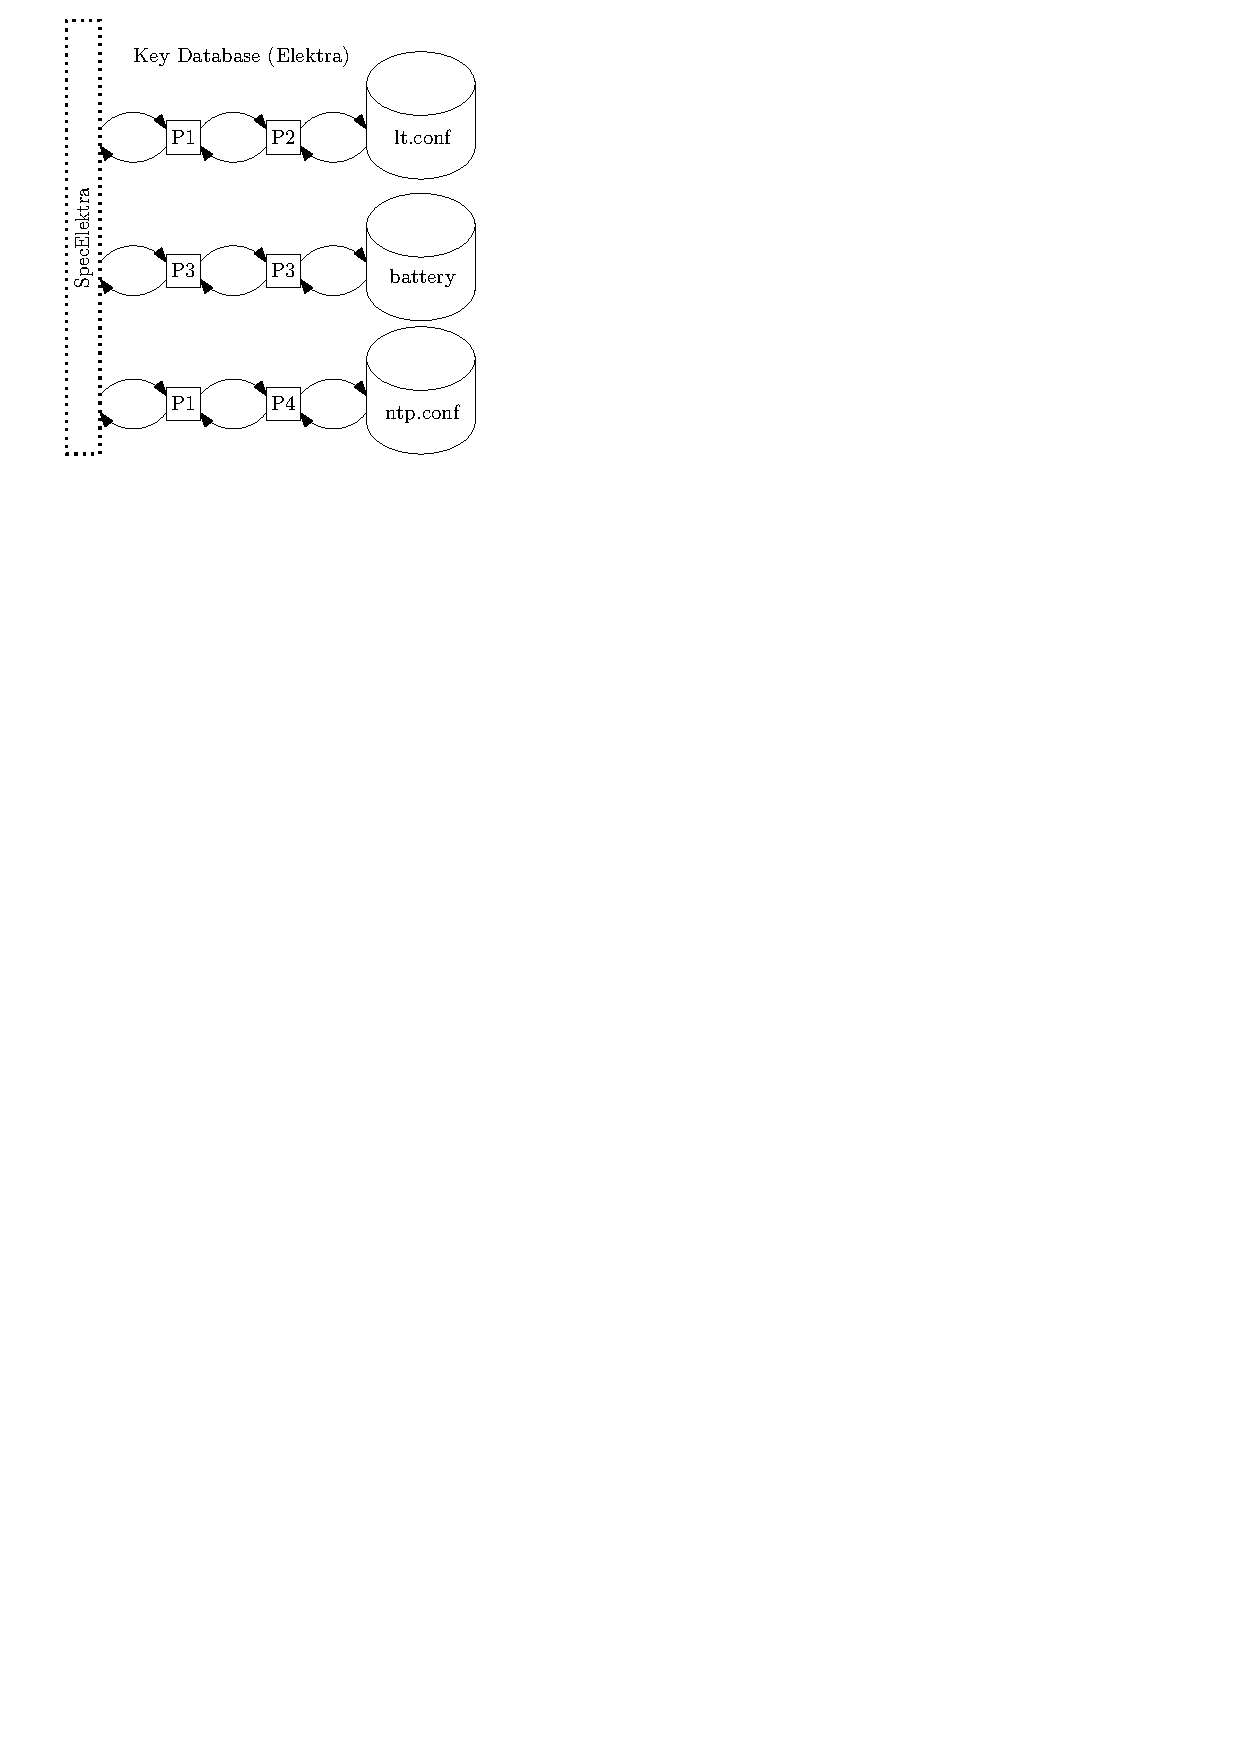
\includegraphics[scale=0.8]{horizontalmodularity}
	\end{column}
	\begin{column}{4cm}
	Cylinders are configuration files, P? are plugins~\cite{raab2016improving}.

	\begin{itemize}
	\item syntax is defined via plugins reading/writing configuration files
	\item semantics are defined via
		\begin{itemize}
		\item plugins interpreting properties
		\item generated code used by applications
		\end{itemize}
	\end{itemize}
	\end{column}
	\end{columns}
\end{frame}

%%%%%%%%%%%%%%%%%%%%%%%%%%%%%%%%%%%%%%%%%% 
\section{Configuration Management}

\begin{frame}[fragile]
	Key/value access in Chef:

	\begin{code}[morekeywords={kdbset,do,action,value,end},gobble=4]
	kdbset 'system/sw/samba/global/workgroup' do
		value 'MY_WORKGROUP'
		action :create
	end
	\end{code}
\end{frame}

\begin{frame}[fragile]
	Key/value access in Ansible:

	\begin{code}[morekeywords={name,connection,key,value,elektra,mountpoint,file,plugins,hosts,tasks},gobble=4]
	- name: setup samba
	  connection: local
	  hosts: localhost
	  tasks:
	  - name: set workgroup
	    elektra:
	      mountpoint: system/sw/samba
	      file: /etc/samba/smb.conf
	      plugins: ini
	    elektra:
	      key: 'system/sw/samba/global/workgroup'
	      value: 'MY_WORKGROUP'
	\end{code}
\end{frame}

\begin{frame}[fragile]
	Key/value access in puppet-libelektra:

	\begin{code}[morekeywords={kdbkey,kdbmount,ensure,value},gobble=4]
	kdbmount {'system/sw/samba':
		ensure => 'present',
		file => '/etc/samba/smb.conf',
		plugins => 'ini'
	}
	kdbkey {'system/sw/samba/global/workgroup':
		ensure => 'present',
		value => 'MY_WORKGROUP'
	}
	kdbkey {'system/sw/samba/global/log level':
		ensure => 'absent'
	}
	\end{code}

	Uniqueness of keys is essential.
	Ideally, applications already mount their configuration at installation.
\end{frame}


\begin{frame}[fragile]
	Key/value specifications in puppet-libelektra:

	\begin{code}[morekeywords={kdbkey,ensure,value},gobble=4]
	kdbkey {'system/sw/samba/global/log level':
		ensure => 'present',
		value => 'MY_WORKGROUP',
		check => {
			'type' => 'short',
			'range' => '0-10',
			'default' => '1',
			'description' => 'Sets the amount of log/
				debug messages that are sent to the
				log file. 0 is none, 3 is consider-
				able.'
	}
	\end{code}

	Ideally, applications already specify their settings.
\end{frame}


%%%%%%%%%%%%%%%%%%%%%%%%%%%%%%%%%%%%%%%%%%%%%%%%%%%%
\section{Problems in Flexibility}

\subsection{Feature Interaction}

\begin{frame}[fragile]
	\frametitle{Fixed Order}

	\begin{code}
	[foo/bar]
	  encrypt:=1
	  zip:=1
	\end{code}

	\begin{itemize}
	\item zip must happen before encrypt
	\item can be specified within plugins
	\end{itemize}
\end{frame}

\begin{frame}[fragile]
	\frametitle{Plugins}

	Plugins that modify the KeySet can be very problematic, e.g. notification:
	\begin{code}[gobble=4]
	[foo/bar]
	  rename/toupper:=1
	  notify:=1
	  type:=string
	\end{code}

	\begin{itemize}
	\item expected: notify on change of key
	\item actual: always notifies because of renaming
	\item ordering does not help, as notification must happen at end
	\end{itemize}
\end{frame}

\subsection{Integration of Operators}

\begin{frame}
	\frametitle{Sum Types}

	\begin{code}[morekeywords={check,type,range,math},gobble=4]
	[a]
	  check/type:=long
	[b]
	  check/type:=long
	[c]
	  check/type:=long
	  check/range:=0-10
	  check/math:="== + a b"
	\end{code}

	\begin{itemize}
	\item ideal to further restrict types
	\item does not work for sum types
	\end{itemize}
\end{frame}

\begin{frame}
	\frametitle{Integration}

	\begin{code}[morekeywords={check,type,range,math},gobble=4]
	[c]
	  check/type:=long
	  check/range:=0-10
	  check/math:="== + a b"
	  check/condition "(a == '3') ? (b == '5')"
	\end{code}

	\begin{itemize}
	\item does not allow math expression to be embedded in condition
	\item temporary variables are needed
	\end{itemize}
\end{frame}


\section{Conclusion}

\begin{frame}
	\frametitle{Conclusion}
	\begin{itemize}
	\item make simple configuration management tasks simple
	\item plugin development needs careful consideration of interactions
	\item operators not always combinable
	\end{itemize}
\end{frame}



%%%%%%%%%%%%%%%%%%%%%%%%%%%%%%%%%%%%%%%%%% 
\nocite{raab2017introducing}

\appendix

\begin{frame}[allowframebreaks]
	\bibliographystyle{plainnat}
	\bibliography{../shared/elektra.bib}
\end{frame}

\end{document}


